%%%%%%%%%%%%%%%%%%%%%%%%%%%%%%%%%%%%%%%%%%%%%%%%%%%%%%%%%%%%
%%%%%%%%%%%%%%%%%%%%%%%%%%%%%%%%%%%%%%%%%%%%%%%%%%%%%%%%%%%%
\section{Introduction}
%%%%%%%%%%%%%%%%%%%%%%%%%%%%%%%%%%%%%%%%%%%%%%%%%%%%%%%%%%%%
%%%%%%%%%%%%%%%%%%%%%%%%%%%%%%%%%%%%%%%%%%%%%%%%%%%%%%%%%%%%

\subsection{Contexte}
-Blabla : objectifs du projets ...
-Rappel des données et des outils
\subsection{Problématique}
-Blabla sur l'actualité
-En fonction des résultats ou bien 
- "Lien entre liberté civile et données démographique, santé, armée, économie, sociale..."?
- Ensuite chercher à trouver (générer) les indices de liberté à partir des résultats (liens, modèles) établis

%%%%%%%%%%%%%%%%%%%%%%%%%%%%%%%%%%%%%%%%%%%%%%%%%%%%%%%%%%%%
%%%%%%%%%%%%%%%%%%%%%%%%%%%%%%%%%%%%%%%%%%%%%%%%%%%%%%%%%%%%
\section{Détermination du champ d'étude}
%%%%%%%%%%%%%%%%%%%%%%%%%%%%%%%%%%%%%%%%%%%%%%%%%%%%%%%%%%%%
%%%%%%%%%%%%%%%%%%%%%%%%%%%%%%%%%%%%%%%%%%%%%%%%%%%%%%%%%%%%
\subsection{Identification des attributs pertinents}
Blabla plus interessant
Cette partie tentera de justifier les choix d'attributs pour leur rapport \emph{possible} avec la liberté civile des peuples.
\subsubsection{Social}
\begin{description}
\item [Adolescent fertility rate] 
Il est possible de supposer --- à la limite --- qu'un état totalitaire aura des particularités du point de vue de la fécondité des adolescents. En effet, on peut imaginer que le taux d'accès aux études supérieures plus bas influence 
\item [Worker's remittances and compensation of employees]
{\huge Je ne sais pas ce que c'est}
\item [Internet users]
Les aspects de censure liés aux dictatures se traduiraient par un usage très limité d'internet. Aussi le nombre d'internautes 
au sein d'une dictature se réduisant aux membres du régime, on s'attend à trouver une relation proportionnelle entre l'indice de liberté et le nombre d'internautes. 
\item [Mobile cellular suscriptions]
Le fort contrôle des moyens de communication de la part d'un régime totalitaire pourrait induire une utilisation de la télphonie mobile très limitée.
\end{description}

\graph{correlation_social}{Corrélation linéaire des différents attributs choisis dans la catégorie \emph{Social}}
Les attributs ayant trait aux nouvelles technologies de l'information sont linéairement corrélés, pour des raisons évidentes. De manière plus surprenante, la fécondité des adolescents semble se rapprocher d'une fonction linéaire décroissante du taux d'accès à Internet\ldots
Sans nous livrer à des conclusions trop hâtives, nous ne considérerons cependant que le taux d'accès Internet en tant qu'attribut représentant les trois.

\subsubsection{Santé}
\begin{description}
\item [Immunization]
Cet attribut est étroitement lié aux impacts de la liberté sur les aspects économiques d'un pays. Un pays totalitaire
accorderait peu d'importance aux achats (imports ?) de vaccins contrairement aux investissements de l'armement militaire.
\item [Life expectancy]
On pourrait croire que les libertés d'un pays influence l'esperance de vie de sa population. Cette hypothèse serait une conséquence
des autres attributs qui lieraient indice de liberté aux aspects économiques et sociales d'un pays. En d'autres termes, moins un pays est libre plus sa situation sociale et sanitaire se dégrade, plus l'espérance de vie décroit.
\item [Mortality rate]
Un pays dépourvu de liberté pourrait avoir un taux de mortalité important dans la mesure où les mouvements des opposants sont réprimés par des peines de mort.
Les engagements militaires d'un tel pays entraineraient des pertes humaines considérables et donc un taux de mortalité élevé.
\item [HIV]
Un indice de liberté très bas augementerait le nombre de personnes atteintes de maladies. En particulier le SIDA.
\end{description}

\graph{correlation_sante}{Corrélation linéaire des différents attributs choisis dans la catégorie \emph{Santé}}
Comme tous les attributs sont corrélés entre eux (on peut trouver au maximum deux attributs ayant un coefficient de corrélation linéaire relativement faible), il est difficile de continuer l'étude sur ce seul groupe d'attributs. Nous verrons par la suite comment remédier à ce problème.

\subsubsection{Armée}
\begin{description}
\item [Adolescent fertility rate]
Cf plus haut.
\item [Military expenditure]
On prévoit de trouver un lien très fort entre les dépenses militaires et l'indice de liberté d'un pays. Un pays totalitaire a de très importants dépenses militaires et inversement.
\item [Fertility rate, total]
On s'attend à trouver un lien entre le taux de fécondité et l'indice de liberté. Un indice de liberté bas se traduirait peut être par un taux de fécondité bas également et inversement.
\item [Life expectancy]
Cf plus haut.
\item [Surface]
Un grand pays en terme de surface pourrait être difficilement controlable par une dictature militaire. Il posséderait donc un indice de liberté plus important qu'un pays plus petit en surface.
\end{description}

\graph{correlation_armee}{Corrélation linéaire des différents attributs choisis dans la catégorie \emph{Armée}}
Sans surprise, le taux de fécondité des adolescentes est fortement lié à celui des femmes en général. De même, l'espérance de vie est fortement liée à ces taux de fécondité. On ne retiendra donc que l'espérance de vie.

\subsubsection{Démographie} 
\begin{description}
\item [Fertility rate]
Cf. plus haut
\item [Adolescent fertility]
Cf. plus haut
\item [Population totale]
On part de la même hypothèse que celle de la surface. Plus la population est importante plus l'indice de liberté est important.
\item Population growth
Tout comme le taux de mortalité, la croissance serait inversement proportionnelle à l'indice de liberté d'un pays.
\item [Life expectancy]
Cf. plus haut
\item [Surface]
Cf. plus haut
\end{description}

\graph{correlation_demographie}{Corrélation linéaire des différents attributs choisis dans la catégorie \emph{Démographie}}
Comme dans le domaine de la santé, les attributs sont corrélés dans des proportions déraisonnables. Ce problème est traité plus bas.

\subsubsection{Economie}
\begin{description}
\item [Agriculture]
Parmi les impacts économiques d'une absence de liberté, on pourrait trouver une très forte participation de l'agriculture dans l'économie d'une dictature militaire.
\item [Export]
On s'attend à trouver une relation inversemment proportionnelle entre la capacité d'une dictature à exporter des services et des biens et l'indice de liberté de celle-ci.
\item [Foreign direct investment]
Idem que pour les exportations. 
\item [GNI per capita, PPP ]
Le revenu national brut pourrait dépendre de l'indice de liberté. Un indice de liberté bas pourrait induire une baisse du revenu national brut.
\item [Imports of goods and services] 
Une dictature militaire, exporterait peu mais importerait de manière importante. notamment les matières première et les produits élémentaires.
\item [Industry, value added]
Au vu des précédentes hypothèses, on pourrait s'attendre à une faible valeur ajoutée industrielle pour une dictature militaire. 
\item [Inflation, GDP deflator] 
On suppose que l'inflation est fortement lié à l'indice de liberté si bien qu'une dictature militaire connaitrait une inflation très importante.
\item [Time required to start a business (days)]
Un indice de liberté bas représente un obstacle aux jeunes entrepreneurs. Aussi, on s'attend à trouver des temps relativement hauts afin de démarrer une nouvelle entreprise. 
\item [Workers remittances and compensation of employees]
Reflet direct du niveau de vie des habitants, cet attribut serait dépendant de l'indice de liberté et s'illustrerait par des salaires et des primes très bas au sein d'une dictature militaire.
\end{description}

\graph{correlation_economie}{Corrélation linéaire des différents attributs choisis dans la catégorie \emph{Economie}}
Cette matrice montre l'importance de la purification des attributs, qui aboutit à la nouvelle matrice suivante.
\graph{correlation_economie_2}{Corrélation linéaire des différents attributs conservés dans la catégorie \emph{Economie}}

\subsubsection{Bilan des choix d'attributs}
Au terme de cette étude des colonnes, nous disposons de 3 jeux d'attributs acceptables --- à la limite. Deux jeux ont dû être éliminés faute d'attributs non corrélés en assez grand nombre. Ces données étant quelque peu limitées, nous tenterons d'utiliser un jeu d'attributs de sémantique hétérogène : constitué du résultat de la PCA de chaque jeu d'attributs, il nous permettra de tenter une autre approche : on essaiera de déterminer les pays libres socialement (ou non) en se basant sur les indices produits par les PCA dans différents domaines : \og social \fg, \og santé \fg, \og armée \fg, \og démographie \fg et \og économie \fg.

\graph{choix_attributs_PCA}{Méthode de construction de l'ensemble d'attributs final}

\subsection{Introduction d'un nouvel attribut}
{\huge TODO}
-Blabla site internet, organisation
-Pb : absence données sous forme de fichiers exploitable directement (cvs) d'ou le script (merci yoyo)

\subsection{Elimination des outliers}
En procédant tout d'abord à une analyse sur chaque dimension, on élimine tout d'abord les premiers et derniers déciles dans chacune d'elles.
\graph{outliers_PCA_avant_1D}{Répartition des pays selon chacune des dimensions obtenues au terme de la PCA}
\graph{outliers_PCA_hilite_1D}{Choix des outliers selon chacune des dimensions obtenues au terme de la PCA}
La tentative d'éliminer plus d'outliers via une analyse en deux dimensions échoue, puisque tous les outliers visibles ont déjà été détectés grâce à l'analyse 1D.
\graph{outliers_PCA_avant_2D}{Choix des outliers selon chaque couple parmis les dimensions obtenues au terme de la PCA}

\subsection{Discrétisation de la dimension \og liberté \fg}
On tente ici de mettre en place un attribut de \og classe \fg, un libellé déterminé par l'indice de liberté. Dans un premier temps, il faut déterminer le nombre de classes à créer. Le noeud \og Hierarchical clustering \fg nous y aide : un optimum de 5 clusters se lit directement sur le graphe suivant.
\graph{distance_liberty_clusters}{Distance entre clusters en fonction du nombre de clusters demandé (clusters hiérarchiques)}
Cette propriété est flagrante sur le dendrogramme.
\graph{hierarchical_liberty_clusters}{Dendrogramme du clustering hiérarchique}

On utilise le même noeud pour nous fournir ces classes. Ceci fait, nous pouvons commencer l'étude proprement dite.

%%%%%%%%%%%%%%%%%%%%%%%%%%%%%%%%%%%%%%%%%%%%%%%%%%%%%%%%%%%%
%%%%%%%%%%%%%%%%%%%%%%%%%%%%%%%%%%%%%%%%%%%%%%%%%%%%%%%%%%%%
\section{Classification non supervisée}
%%%%%%%%%%%%%%%%%%%%%%%%%%%%%%%%%%%%%%%%%%%%%%%%%%%%%%%%%%%%
%%%%%%%%%%%%%%%%%%%%%%%%%%%%%%%%%%%%%%%%%%%%%%%%%%%%%%%%%%%%
On tente ensuite de réaliser trois types de clusterings différents sur les attributs choisis. Ceci en espérant que ces clusters correspondront aux classes de liberté, ce qui est mesuré grâce au noeud \og Entropy Scorer \fg.
\begin{figure}[H]
	\centering
	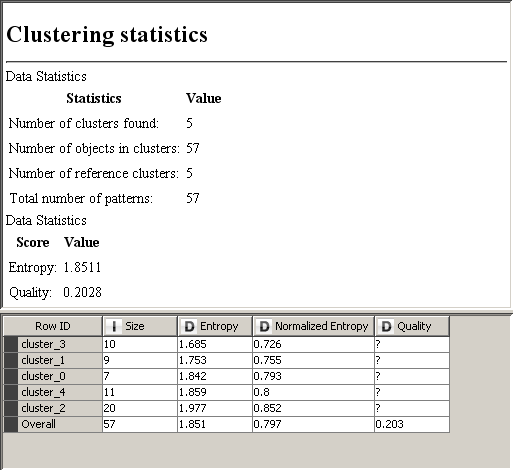
\includegraphics[width=0.3\textwidth]{entropy_hierarchical}
	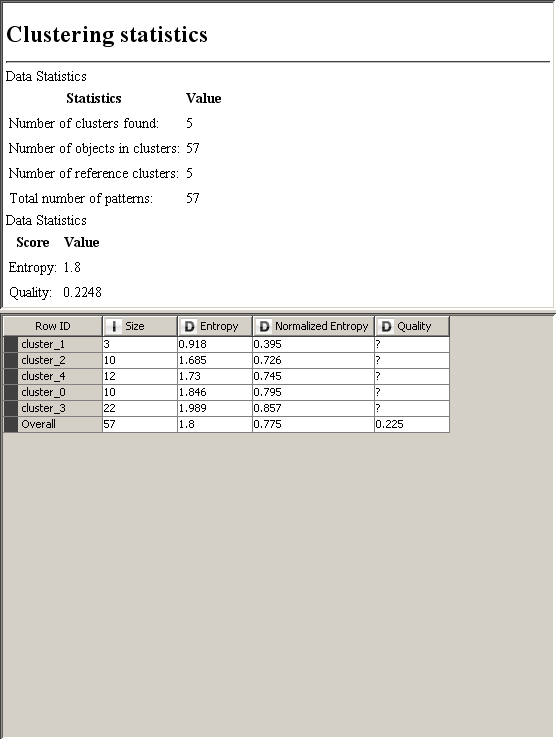
\includegraphics[width=0.3\textwidth]{entropy_fuzzycmeans}
	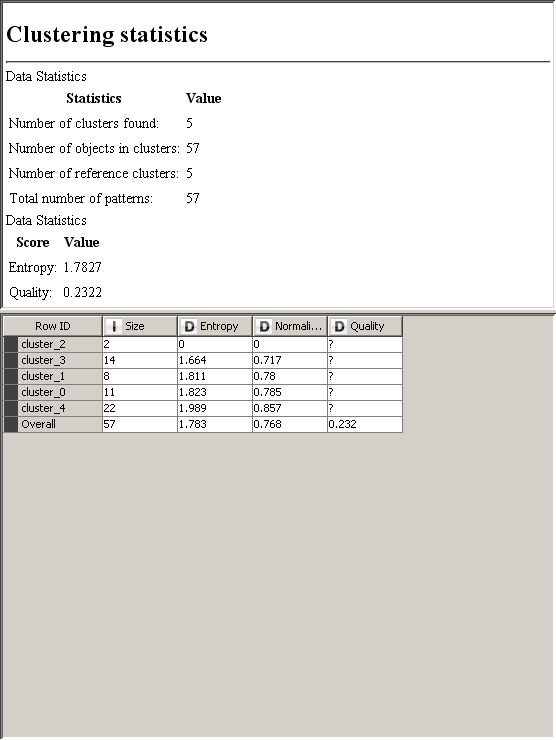
\includegraphics[width=0.3\textwidth]{entropy_kmeans}
	\caption{Mesure de l'entropie des différents clusterings avec les classes de références}
\end{figure}
C'est un échec. L'entropie est clairement énorme et nous montre que le jeu d'attributs choisi ne constitue pas une base intéressante pour déterminer l'indice de liberté : son clustering n'aboutit à rien de semblable aux classes de liberté. En procédant sur les jeux d'attributs \og acceptables à la limite \fg vus plus haut (\emph{Social}, \emph{Armée} et \emph{Economie}), on aboutit au même type de résultats.

%%%%%%%%%%%%%%%%%%%%%%%%%%%%%%%%%%%%%%%%%%%%%%%%%%%%%%%%%%%%
%%%%%%%%%%%%%%%%%%%%%%%%%%%%%%%%%%%%%%%%%%%%%%%%%%%%%%%%%%%%
\section{Classification supervisée}
%%%%%%%%%%%%%%%%%%%%%%%%%%%%%%%%%%%%%%%%%%%%%%%%%%%%%%%%%%%%
%%%%%%%%%%%%%%%%%%%%%%%%%%%%%%%%%%%%%%%%%%%%%%%%%%%%%%%%%%%%






%%%%%%%%%%%%%%%%%%%%%%%%%%%%%%%%%%%%%%%%%%%%%%%%%%%%%%%%%%%%
%%%%%%%%%%%%%%%%%%%%%%%%%%%%%%%%%%%%%%%%%%%%%%%%%%%%%%%%%%%%
\section{Conclusion}
%%%%%%%%%%%%%%%%%%%%%%%%%%%%%%%%%%%%%%%%%%%%%%%%%%%%%%%%%%%%
%%%%%%%%%%%%%%%%%%%%%%%%%%%%%%%%%%%%%%%%%%%%%%%%%%%%%%%%%%%%


